\documentclass{article}
\usepackage{graphicx}
\usepackage{subcaption}
\usepackage{geometry}
\usepackage{tikz}
\usepackage{amsmath}
\usepackage{cleveref}
\usepackage{float}
\usepackage[useregional]{datetime2}
\usepackage{url}
\def\checkmark{\tikz\fill[scale=0.4](0,.35) -- (.25,0) -- (1,.7) -- (.25,.15) -- cycle;}
\usepackage[font=small,skip=0pt]{caption}
\geometry{legalpaper, margin=1in}
\title{Exploratory Analysis of MPG Data Set}
\author{Zhijia Chen}
\date{\today}

\begin{document}

\begin{titlepage}
    \maketitle
\end{titlepage}

On October 19, 1973, the Organization of Arab Petroleum Exporting Contries (OPEC) imposed an oil embargo targeted at nations perceived as supporting Israel during the Yom Kippur War~\cite{smith2004palestine}. That embargo caused a global oil crisis and was later called the "first oil shock". During the oil crisis, the oil price had risen almost 300\% from \$3 per barrel to nearly \$12 globally[Oil Embargo, 1973–1974]. As a measure to reduce energy consumption and improve nation's energy security, the congress passed Corporated Average Fuel Economy (CAFE) Standards in 1975~\cite{CAFE}. The CAFE standards regulates the minium milegage per galon (MPG) that must be achieved by all automakers for their cars and trucks each year since 1978. The regulation pushes automakers to make more efficient cars year by year. Between 1975 and 1985, average passenger vehicle mileage doubled from about 13.5 mpg to 27.5~\cite{to54.5MPG}. But an ineresting question is, how do automakers achieve that? By auto technology advancement alone, or by making performance compromise? In this exploratory aalysis, we will exame the MPG dataset and try to get some insight about this question.

We first check how the MPG changed before and after the enforcement of CAFE. Figure~\ref{yearly-MPG-CAFE} shows the boxplot of MPG grouped by model year between 1970 and 1982, and the yellow line shows the average MPG while the red line with star markers shows the CAFE standards since 1978. Clearly, the average MPG has increased steadily before the "first oil shock", without the regulation mandate. However, the gap between the minimum value and the first quartile is increaing, which implies the regulation does drive some automakers that lag behind average to make more efficient cars.

\begin{figure}[h!]
    \centering
    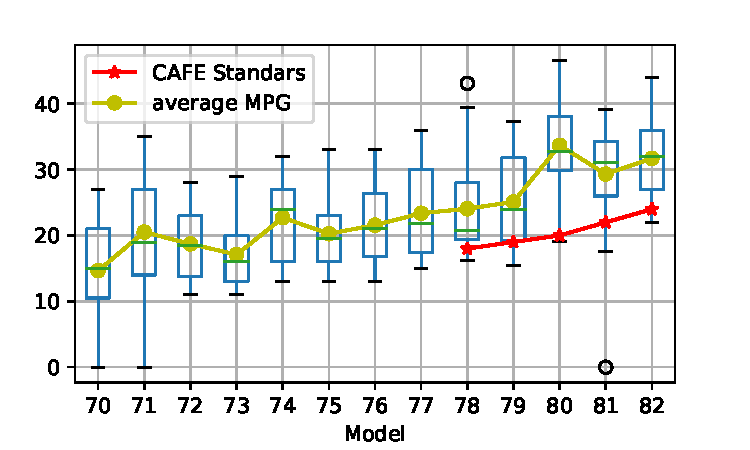
\includegraphics{yearly-MPG-CAFE.pdf}
    \caption{MPG boxplot grouped by model.}
    \label[fig]{yearly-MPG-CAFE}
\end{figure}

To study if automakers make any performance compromise to improve MPG, we will look into two key prameters: horsepower and acceleration. Figure~\ref{mpg-scatter} shows the MPG scatter plot with horsepower (left) and acceleration (right) respectively. Intrestingly, horsepower tends to decrease as MPG increases, which could imply that automakers sacrifice engine powers in favor of higher MPG. However, The acceleration actually positively correlated with MPG, meaning that cars run faster with higher MPG.

\begin{figure}[h!]
    \centering
    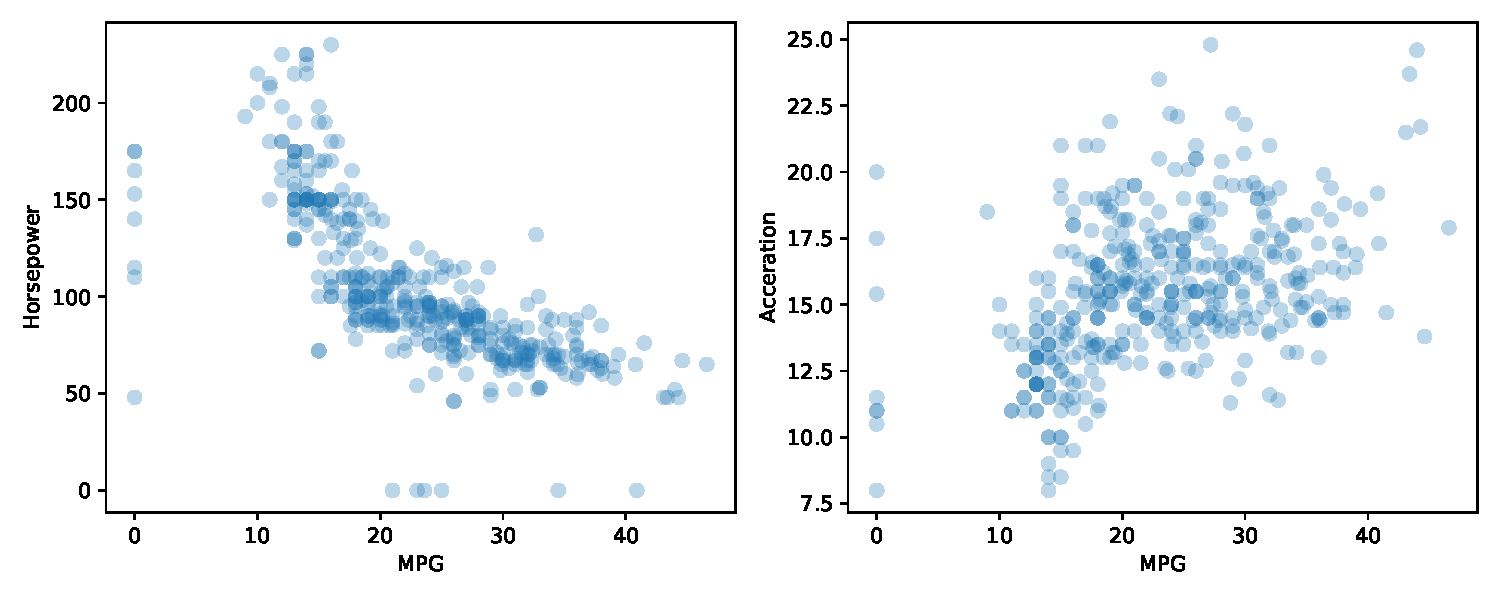
\includegraphics[width=1\linewidth]{MPG-Horsepower-Acceleration.pdf}
    \caption{MPG scatter plot with Horsepower and Acceleration.}
    \label[fig]{mpg-scatter}
\end{figure}

The fact seems somewhat counter intuitive, as faster acceleration usually requires higher power. But still, this could be explained by two reasons:
\begin{enumerate}
    \item Automakers are able to reduce car weight to compensate the horsepower reduction and even achieved faster acceleration. 
    \item The technology advancement enable automakers to produce more efficient car so that acceleration is increased even with lower horsepower.
\end{enumerate} 
Note that $a=\sqrt{\frac{P\eta}{2mt}}$, where $a$, $P$, $m$ and $t$ are acceleration, horsepower, weight and time respectively. And $\eta$ is the overall efficiency factor.

We will first study the change of car weight in this period. Figure~\ref{yearly-weight} shows the average car weight and average acceleration of each year. We see that, overall speaking, the car weight dose decrease overtime, and the two parameters prensent a clear opposite trend except for the year of 75, 76 and 77 when they both decrease. This proves that car weight is a key parameters targeted by automakers to improve MPG and acceleration. 

\begin{figure}[h!]
    \centering
    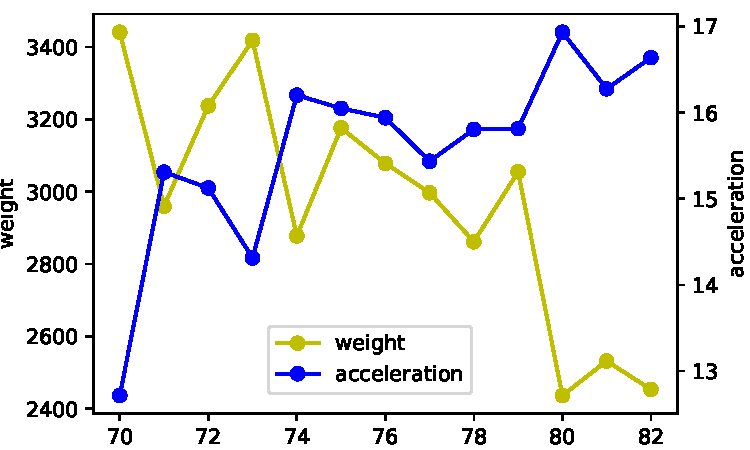
\includegraphics{yearly-weight.pdf}
    \caption{Weight boxplot grouped by model.}
    \label[fig]{yearly-weight}
\end{figure}

There is no parameters to show the efficiency factor directly, so we try to exame if weight is a dominant factor that improves MPG. We group cars by the number of cylinders, and for each pair of cars $c_i$, $c_j$ in a group , we compute a tuple $(x, y)$ where
\begin{align*}
    weight(c_i) &>=weight(c_j)\\
    x&=weight(c_i)-weight(c_j)\\
    y&=MPG(c_j)-MPG(c_i)
\end{align*}
If weight is a dominant factor in improving MPG, then most of the points should be located in the first quadrant. Figure~\ref{diff-weight-mpg} presents the distribution of the points. We see that most of points are located in the first quadrant, so we get the conclusion that the main factor that contributes to higher MPG is car weight. 

\begin{figure}[h!]
    \centering
    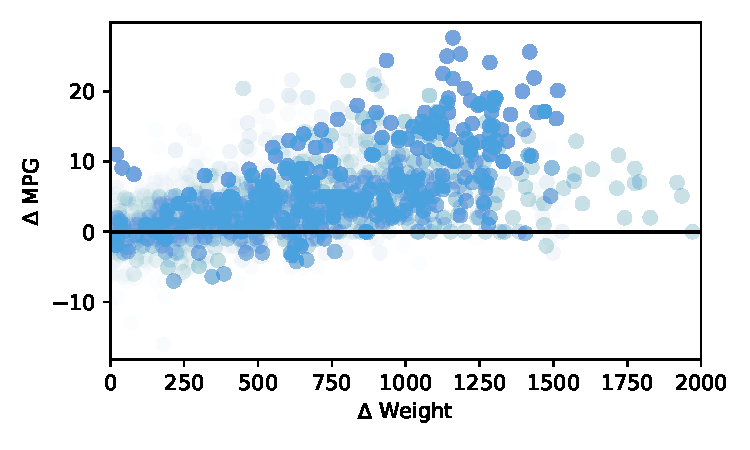
\includegraphics{diff-MPG-Weight.pdf}
    \caption{$\Delta$ Weight vs $\Delta$ MPG}
    \label[fig]{diff-weight-mpg}
\end{figure}

\bibliography{assignment1} 
\bibliographystyle{ieeetr}
\end{document}

